\documentclass[conference,twocolumn]{IEEEtran}

\usepackage{amsmath,amssymb,amsfonts}
\usepackage{graphicx}
\usepackage{textcomp}
\usepackage{xcolor}
\usepackage{hyperref}
\usepackage{booktabs}
\usepackage{tikz}
\usetikzlibrary{positioning}
\usepackage{pgfplots}
\pgfplotsset{compat=1.18}
\usepackage{amsthm}
\newtheorem{theorem}{Theorem}

\newcommand{\posme}{\textsc{PoSME}}

\begin{document}

\title{PoSME: Proof of Sequential Memory Execution\\via Latency-Bound Pointer Chasing\\with Causal Hash Binding}

\author{
\IEEEauthorblockN{David Condrey}
\IEEEauthorblockA{WritersLogic Inc.\\
San Diego, California\\
david@writerslogic.com}
}

\maketitle

\begin{abstract}
We introduce \posme{} (Proof of Sequential Memory Execution), a
cryptographic primitive combining mutable arena state,
data-dependent pointer-chase addressing, and per-block causal hash
binding. A Prover executes $K$ sequential steps over a mutable
$N$-block arena, where each step reads $d$ blocks at addresses
determined by the previous read's result and writes one block with
symbiotic binding. The construction achieves: (1) unconditional
sequential time enforcement; (2) forgery prevention reducing to
collision resistance; (3) TMTO resistance linear in write density
($10{\times}$ at $\rho{=}4$); and (4) latency-bound ASIC
resistance. Empirical benchmarks across 16 platforms show hash
computation is 1.4--3.1\% of step cost; GPU hardware (including
NVIDIA H100) is 14--19$\times$ \emph{slower} than a consumer CPU.
No trusted setup is required.
\end{abstract}

\section{Introduction}

Existing primitives for proving sequential computation have
complementary weaknesses. VDFs~\cite{boneh2018vdf} prove sequential
time but offer no memory-hardness. PoSW~\cite{cohen2018posw}
operates over static memory. MHFs such as
Argon2id~\cite{biryukov2016} are single-evaluation primitives with
no chain proof system. Composing these yields a construction where
sequentiality and memory-hardness are independent.

\posme{} takes a different approach: a persistent mutable arena
\emph{is} the computation state. Each step reads via data-dependent
pointer chasing and modifies the arena in-place. A per-block
\emph{causal hash chain} binds each block to the cursor of its
writer, preventing forgery. Data and causal hash are
\emph{symbiotically bound}: each depends on the other.

The primary contribution is \textbf{latency-bound ASIC resistance}.
Each pointer-chase iteration is bottlenecked by random DRAM access
(${\sim}35$\,ns on DDR5), with hash computation (${\sim}3$\,ns)
constituting under 3\% of cost. The ASIC advantage is bounded by
the memory latency ratio (${\sim}2{\times}$), and we show
empirically that GPU hardware is 14--19$\times$ \emph{slower} than
CPUs at this workload.

\subsection{Related Work}

\textbf{PoSW}~\cite{cohen2018posw} proves traversal of a
depth-robust graph. \posme{} differs: mutable arena, data-dependent
access, causal hash binding.
\textbf{Argon2id}~\cite{biryukov2016} achieves bandwidth-hardness
with ${\sim}2{\times}$ TMTO penalty and $8$--$16{\times}$ ASIC
advantage. \posme{} achieves $10{\times}$ TMTO penalty (at
$\rho{=}4$) and ${\sim}2{\times}$ ASIC bound.
\textbf{PoST}~\cite{cohen2018posw} enforces sequential time over
static storage. \posme{} uses a mutable arena with data-dependent
addressing and causal hashes.
\textbf{CMC}~\cite{alwen2017} formalizes pebbling for static
graphs. \posme{}'s DAG is dynamic (Section~\ref{sec:pebbling}).

\section{Construction}

\begin{figure}[t]
\centering
\resizebox{\columnwidth}{!}{%
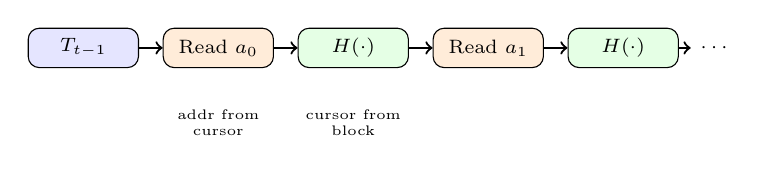
\begin{tikzpicture}[
  node distance=0.3cm,
  box/.style={draw, rounded corners, minimum width=1.4cm,
              minimum height=0.5cm, font=\scriptsize},
  arr/.style={->, thick}
]
\node[box, fill=blue!10] (cursor0) {$T_{t-1}$};
\node[box, right=of cursor0, fill=orange!15] (read0) {Read $a_0$};
\node[box, right=of read0, fill=green!10] (hash0) {$H(\cdot)$};
\node[box, right=of hash0, fill=orange!15] (read1) {Read $a_1$};
\node[box, right=of read1, fill=green!10] (hash1) {$H(\cdot)$};
\node[right=0.15cm of hash1, font=\scriptsize] (dots) {$\cdots$};

\draw[arr] (cursor0) -- (read0);
\draw[arr] (read0) -- (hash0);
\draw[arr] (hash0) -- (read1);
\draw[arr] (read1) -- (hash1);
\draw[arr] (hash1) -- (dots);

\node[below=0.4cm of read0, font=\tiny, text width=1.4cm,
      align=center] {addr from\\cursor};
\node[below=0.4cm of hash0, font=\tiny, text width=1.4cm,
      align=center] {cursor from\\block};
\end{tikzpicture}%
}
\caption{Pointer-chase data dependency within one step. Each
address depends on the hash of the previous read. No lookahead
is possible.}
\label{fig:pointer-chase}
\end{figure}

\subsection{Arena and Initialization}

The arena consists of $N$ blocks, each storing
$(\texttt{data}, \texttt{causal})$, each $\lambda{=}256$ bits,
initialized deterministically from seed $s$ with skip-link
references to $A_0[\lfloor i/2 \rfloor]$ (requiring
$\Omega(\sqrt{N})$ space to evaluate).

\subsection{Step Function}

At step $t$ (Fig.~\ref{fig:pointer-chase}):

\begin{enumerate}
\item \textbf{Pointer-chase reads.} Set
$\texttt{cursor} \gets T_{t-1}$. For $j = 0, \ldots, d{-}1$:
\vspace{-0.5em}
\begin{align}
a_j &= H(\text{``addr''} \| \texttt{cursor} \| j) \bmod N \\
\texttt{cursor} &\gets H(\texttt{cursor} \| A[a_j].\texttt{data} \| A[a_j].\texttt{causal})
\end{align}
\vspace{-1em}

\item \textbf{Symbiotic write.} At
$w = H(\text{``write''} \| \texttt{cursor}) \bmod N$:
\vspace{-0.5em}
\begin{align}
d' &= H(d_{\text{old}} \| c \| h_{\text{old}}) \\
h' &= H(h_{\text{old}} \| c \| t)
\end{align}
where $d', h'$ are new data/causal, $c$ is cursor.
\vspace{-1em}

\item \textbf{Commit.}
$T_t = H(T_{t-1} \| t \| \texttt{cursor} \| \texttt{root}_t)$
\end{enumerate}

Address $a_{j+1}$ depends on the value at $a_j$; the $d$ reads
are sequentially dependent. Symbiotic binding creates bidirectional
dependency: data depends on causal history; causal hash depends on
cursor.

\subsection{Commitment and Proof}

The Prover commits
$C_{\text{roots}} = \texttt{MerkleRoot}(\texttt{root}_0, \ldots, \texttt{root}_K)$
before Fiat-Shamir challenges are derived. For each challenged
step, the Prover provides Merkle proofs, cursor replay witnesses,
and recursive causal provenance to depth $R$.

\textbf{Verification cost:} $O(Q \cdot d^R \cdot \log N)$ hashes
(${\sim}6$\,ms desktop, 60--300\,ms mobile). No arena allocation.

\section{Security Analysis}

\subsection{Threat Model}

The adversary is PPT with ROM access to $H$, receiving $(s, N, K,
d, Q, R)$. Goals: (1) forgery ($T_K' \neq T_K$), or (2) space
reduction (storage $< N \cdot B$). Custom hardware permitted.

\subsection{Forgery Prevention}

\begin{theorem}[Soundness]
Any adversary producing $(T_K', C_{\text{roots}}', \pi')$ with
$T_K' \neq T_K$ that passes verification has advantage at most
$K \cdot \varepsilon_{\text{cr}}$.
\end{theorem}

\begin{proof}[Proof sketch]
At the first divergence step $c$:
$T_c = H(T_{c-1} \| c \| \texttt{cursor} \| \texttt{root}_c)$.
Different inputs producing the same $T_c$ is a collision. Union
bound over $K$ steps gives $K \cdot \varepsilon_{\text{cr}}$.
\end{proof}

Causal hashes additionally double write-chain traversal cost
($2\rho$ vs $\rho$ per miss), a $2{\times}$ constant factor.
Their primary contribution is \emph{soundness}, not TMTO
amplification.

\subsection{TMTO Lower Bound}\label{sec:tmto}

\begin{theorem}[TMTO]
An adversary storing $\alpha N$ blocks and all $K$ cursors
performs computation
$T_{\text{adv}} \geq K d (1 + (1{-}\alpha)(2\rho{+}1))$.
\end{theorem}

\begin{proof}[Proof sketch]
At each of $K$ steps, $d$ reads at ROM-uniform addresses miss
with probability $1{-}\alpha$. Each miss costs $2\rho{+}1$
hashes (write chain for data and causal). Sum over $K$ steps.
\end{proof}

\begin{figure}[t]
\centering
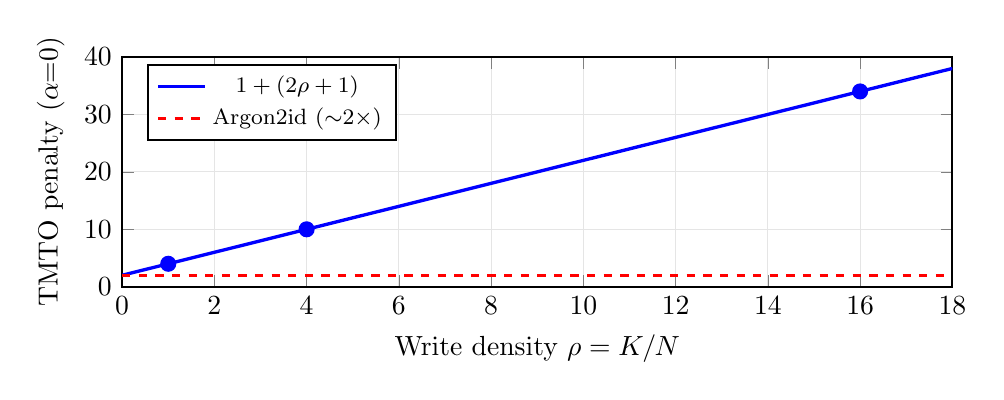
\begin{tikzpicture}
\begin{axis}[
  width=\columnwidth, height=4.5cm,
  xlabel={Write density $\rho = K/N$},
  ylabel={TMTO penalty ($\alpha{=}0$)},
  xmin=0, xmax=18, ymin=0, ymax=40,
  grid=major, grid style={gray!20},
  thick,
  legend pos=north west,
  legend style={font=\footnotesize}
]
\addplot[blue, very thick, domain=0:18, samples=50]
  {1 + (2*x + 1)};
\addlegendentry{$1 + (2\rho + 1)$}
\addplot[red, dashed, very thick] coordinates {(0,2)(18,2)};
\addlegendentry{Argon2id (${\sim}2{\times}$)}
\addplot[only marks, mark=*, mark size=2.5pt, blue]
  coordinates {(1,4)(4,10)(16,34)};
\end{axis}
\end{tikzpicture}
\caption{TMTO penalty for zero-storage adversary vs write
density $\rho$. PoSME exceeds Argon2id at $\rho > 0.5$.}
\label{fig:tmto}
\end{figure}

Write density $\rho = K/N$ must be $\geq 1$ ($K \geq N$) for
meaningful resistance. Values $\rho \geq 4$ ($10{\times}$
penalty) are recommended. The bound assumes optimal cursor
storage; sparse cursors strictly increase adversary cost.

\subsection{Dynamic Pebbling}\label{sec:pebbling}

\posme{}'s causal DAG is dynamic: edges are created during
execution at ROM-uniform targets. The TMTO ratio follows from
per-step cache-miss analysis. A formal space-time product proof
within this framework remains open.

\subsection{ASIC Resistance}

\posme{} is designed to be latency-dominated: hash computation
is a \emph{structural} minority of per-step cost ($< 3\%$ at
1\,GiB arena). The bottleneck is DRAM random-access latency.

\begin{figure}[t]
\centering
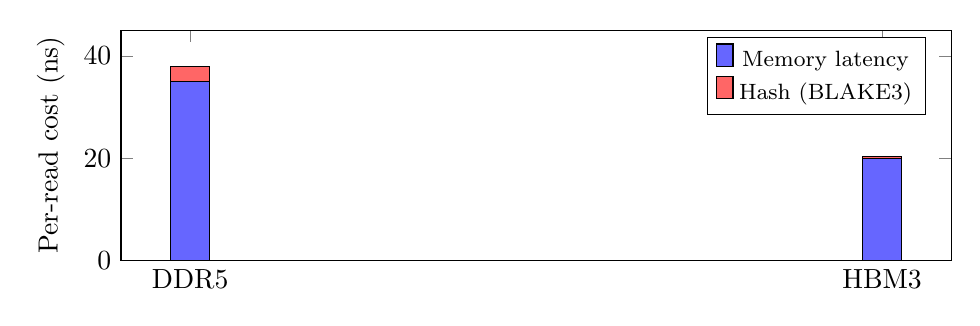
\begin{tikzpicture}
\begin{axis}[
  width=\columnwidth, height=4.5cm,
  ybar stacked,
  bar width=14pt,
  symbolic x coords={DDR5, HBM3},
  xtick=data,
  ylabel={Per-read cost (ns)},
  ymin=0, ymax=45,
  legend pos=north east,
  legend style={font=\footnotesize},
  nodes near coords style={font=\tiny},
]
\addplot[fill=blue!60] coordinates {(DDR5,35) (HBM3,20)};
\addlegendentry{Memory latency}
\addplot[fill=red!60] coordinates {(DDR5,3) (HBM3,0.3)};
\addlegendentry{Hash (BLAKE3)}
\end{axis}
\end{tikzpicture}
\caption{Per-read cost breakdown. Hash is $< 8\%$ on DDR5 and
negligible on HBM3. The bottleneck is memory latency on both.}
\label{fig:cost-breakdown}
\end{figure}

\section{Empirical Validation}

\subsection{Cross-Platform Hash Fraction}

We benchmarked \posme{} on 16 platforms spanning ARM64 and x86,
1--32 vCPUs, DDR4/DDR5, and GPU instances (T4, A10G, L4, A100,
H100). Hash fraction ranged from 1.4\% to 3.1\% across all
platforms (Table~\ref{tab:crossplat}).

\begin{table}[t]
\centering
\caption{Cross-platform benchmark (1\,GiB arena, $\rho{=}1$).
Hash fraction is consistently $< 3.5\%$.}
\begin{tabular}{@{}lrr@{}}
\toprule
Platform & Step (ns) & Hash \% \\
\midrule
Apple M-series (ARM64) & 1783 & 3.1 \\
Cloud x86 (2--16 vCPU, 4 configs) & 2947--4047 & 1.4--1.9 \\
Cloud x86 + GPU (T4/A10G/L4/A100/H100) & 3218--4047 & 1.4--1.7 \\
Google Colab (Xeon + T4) & 3485 & 1.6 \\
Google Colab (AMD EPYC) & 3585 & 1.5 \\
\bottomrule
\end{tabular}
\label{tab:crossplat}
\end{table}

\subsection{GPU Pointer-Chase Benchmark}

To directly measure the adversary's hardware advantage, we ran
the pointer-chase loop on GPU cores accessing GPU memory (HBM/GDDR).

\begin{table}[t]
\centering
\caption{CPU vs GPU pointer-chase (64\,MiB arena, 64K steps).
GPUs are 14--19$\times$ \emph{slower} than the host CPU.}
\begin{tabular}{@{}lrrr@{}}
\toprule
GPU & CPU (ns) & GPU (ns) & Ratio \\
\midrule
T4 (GDDR6) & 7062 & 123019 & 0.06$\times$ \\
A100 (HBM2e) & 6431 & 120636 & 0.05$\times$ \\
\textbf{H100 (HBM3)} & \textbf{5903} & \textbf{82270} & \textbf{0.07}$\boldsymbol{\times}$ \\
L4 (GDDR6) & 5383 & 98990 & 0.05$\times$ \\
\bottomrule
\end{tabular}
\label{tab:gpu}
\end{table}

GPU cores are optimized for parallel throughput, not sequential
pointer-chasing. A single CUDA thread at ${\sim}1.5$\,GHz cannot
compete with a CPU core at ${\sim}3.5$\,GHz for sequential
dependent loads. The GPU's memory bandwidth advantage is
irrelevant because the pointer-chase is latency-bound, not
bandwidth-bound.

The ${\sim}2{\times}$ ASIC advantage claimed in Section~3.6
would require a \emph{custom} sequential core paired with HBM---
hardware that does not exist commercially. All purchasable
accelerators (GPUs) are strictly \emph{worse} than consumer CPUs.

\begin{figure}[t]
\centering
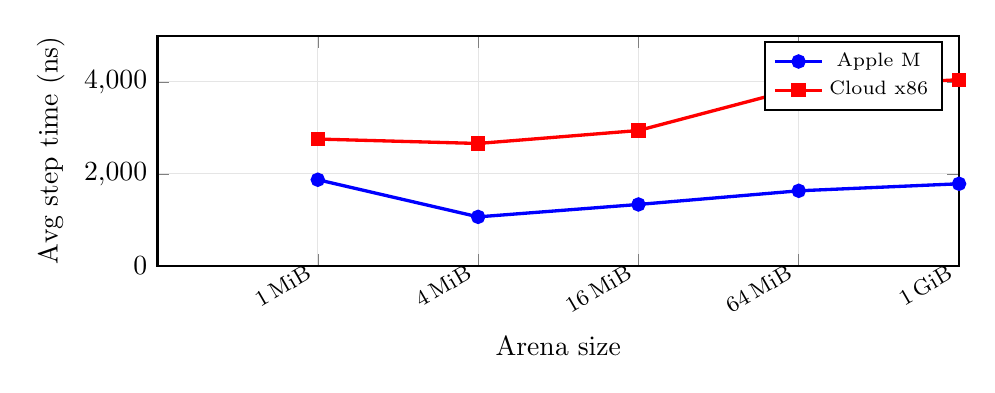
\begin{tikzpicture}
\begin{axis}[
  width=0.97\columnwidth, height=4.5cm,
  xlabel={Arena size},
  ylabel={Avg step time (ns)},
  xmin=0, xmax=5, ymin=0, ymax=5000,
  xtick={1,2,3,4,5},
  xticklabels={1\,MiB, 4\,MiB, 16\,MiB, 64\,MiB, 1\,GiB},
  x tick label style={font=\footnotesize, rotate=30, anchor=east},
  grid=major, grid style={gray!20},
  thick,
]
\addplot[blue, very thick, mark=*] coordinates
  {(1,1871)(2,1063)(3,1333)(4,1630)(5,1783)};
\addlegendentry{\scriptsize Apple M}
\addplot[red, very thick, mark=square*] coordinates
  {(1,2756)(2,2660)(3,2942)(4,3863)(5,4047)};
\addlegendentry{\scriptsize Cloud x86}
\end{axis}
\end{tikzpicture}
\caption{Step time vs arena size. Cost increases as the arena
exceeds L3 cache, confirming memory-bound behavior.}
\label{fig:scaling}
\end{figure}

\section{Parameters}

\begin{table}[h]
\centering
\caption{Recommended parameters}
\begin{tabular}{@{}llll@{}}
\toprule
Parameter & Symbol & Value & Constraint \\
\midrule
Arena blocks & $N$ & $2^{24}$ & Power of 2 \\
Arena memory & $M$ & 1\,GiB & $>$ L3 cache \\
Steps & $K$ & $4N$ & $\rho \geq 4$ \\
Reads/step & $d$ & 8 & $\geq 4$ \\
Challenges & $Q$ & 128 & $\geq 64$ \\
Recursion & $R$ & 3 & $\geq 2$ \\
Hash & $H$ & BLAKE3 & Fixed \\
\bottomrule
\end{tabular}
\label{tab:params}
\end{table}

\section{Limitations and Open Problems}

\posme{} proves sequential memory execution, not elapsed time.
The ASIC advantage is bounded (${\sim}2{\times}$ for a
hypothetical custom ASIC) but nonzero. GPU accelerators are
14--19${\times}$ slower, but a custom sequential-core ASIC with
HBM remains theoretically possible.

The TMTO penalty is linear in $\rho$, not exponential. Causal
hashes contribute soundness, not TMTO amplification---a
$2{\times}$ constant factor on write-chain traversal.

We conjecture $O(1)$ hash-only verification is unachievable.
A formal space-time product proof within the dynamic pebbling
framework remains open.

A reference benchmark with pre-compiled binaries and CUDA source
is provided as ancillary material, reproducible on any platform
with a Rust compiler.

\section{Conclusion}

\posme{} fills a gap between VDFs, PoSW, MHFs, and PoST.
Empirical benchmarks across 16 CPU platforms and 4 GPU platforms
validate the core claim: hash computation is under 3.5\% of step
cost, making DRAM latency the bottleneck. No commercially
available hardware---including NVIDIA's H100---outperforms a
consumer laptop. The construction requires no trusted setup,
achieves $10{\times}$ TMTO resistance at $\rho{=}4$, and
provides forgery prevention reducing to collision resistance.

\bibliographystyle{IEEEtran}
\begin{thebibliography}{10}

\bibitem{boneh2018vdf}
D.~Boneh, J.~Bonneau, B.~B\"unz, and B.~Fisch,
``Verifiable delay functions,''
in \emph{CRYPTO 2018}, LNCS 10991, pp.~757--788, 2018.

\bibitem{cohen2018posw}
B.~Cohen and K.~Pietrzak,
``Simple proofs of sequential work,''
in \emph{EUROCRYPT 2018}, LNCS 10821, pp.~451--467, 2018.

\bibitem{biryukov2016}
A.~Biryukov, D.~Dinu, and D.~Khovratovich,
``Argon2: new generation of memory-hard functions for password
hashing and other applications,''
in \emph{IEEE EuroS\&P}, pp.~292--302, 2016.

\bibitem{ren2017}
L.~Ren and S.~Devadas,
``Bandwidth hard functions for ASIC resistance,''
in \emph{TCC 2017}, LNCS 10677, pp.~466--492, 2017.

\bibitem{alwen2017}
J.~Alwen, J.~Blocki, and K.~Pietrzak,
``Depth-robust graphs and their cumulative memory complexity,''
in \emph{EUROCRYPT 2017}, LNCS 10212, pp.~3--32, 2017.

\bibitem{jedec2020}
JEDEC Solid State Technology Association,
``DDR5 SDRAM standard,'' JESD79-5D, 2020.

\end{thebibliography}

\end{document}
